\documentclass{standalone}
\usepackage{tikz}
\usepackage{mathtools}
\usepackage{pgfplots}

\pgfplotsset{compat=newest}

\definecolor{color1}{RGB}{255,158,1}
\definecolor{color2}{RGB}{255,74,1}
\definecolor{color3}{RGB}{220,0,0}

\begin{document}
    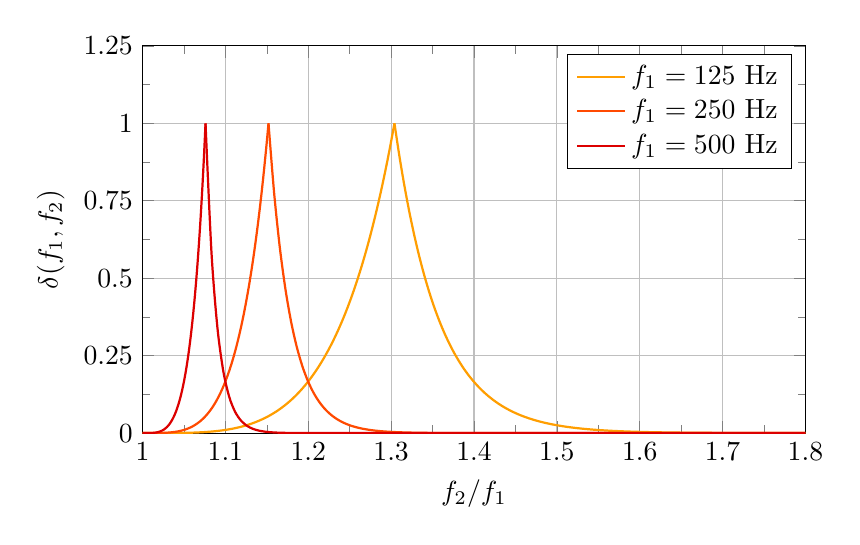
\begin{tikzpicture}
        \begin{axis}[
            xmin = 1, xmax = 1.8, %
            ymin = 0, ymax = 1.25, %
            xtick distance = 0.1, %Is the distance between major ticks in the x-axis.
            ytick distance = 0.25, %Is the distance between major ticks in the y-axis.
            grid = major, %When this options is set to both the minor and major grid are plotted.
            minor tick num = 1, %Is the number of ticks between major ticks.
            major grid style = {lightgray}, %Changes the color and stroke of the major grid.
            width = 10cm, %sets the width of the figure
            height = 6.5cm,  %sets the height of the figure
            xlabel = {$f_2/f_1$}, %
            ylabel = {$\delta(f_1,f_2)$}, %
            legend cell align = {left}, %
        ]
        
        %%%%%%%%%%%%%%%% Frequency1 %%%%%%%%%%%%%%%%
            \addplot[
                domain=1:1.304, %Domain of the fucntion
                samples=200, %This parameter determines the number of point to be plotted for the function, while bigger the number better looks the function.
                smooth, %f we use this option, the compiler makes an interpolation between the point plotted to get a soft appearance for the function.
                thick, %Stroke of the function. Options: ultra thin, very thin, thin, semithick, thick, very thick, ultra thick.
                color1 %Color of the function.
            ]{cosh(14.2503*(x-1)^2)-1};
            \addplot[
                domain=1.304:2.5, %Domain of the fucntion
                samples=200, %This parameter determines the number of point to be plotted for the function, while bigger the number better looks the function.
                smooth, %f we use this option, the compiler makes an interpolation between the point plotted to get a soft appearance for the function.
                thick, %Stroke of the function. Options: ultra thin, very thin, thin, semithick, thick, very thick, ultra thick.
                color1 %Color of the function.
            ]{exp(-0.15*125*(x-1-38/125)};
            
            
            %%%%%%%%%%%%%%%% Frequency2 %%%%%%%%%%%%%%%%
            \addplot[
                domain=1:1.152, %Domain of the fucntion
                samples=200, %This parameter determines the number of point to be plotted for the function, while bigger the number better looks the function.
                smooth, %f we use this option, the compiler makes an interpolation between the point plotted to get a soft appearance for the function.
                thick, %Stroke of the function. Options: ultra thin, very thin, thin, semithick, thick, very thick, ultra thick.
                color2 %Color of the function.
            ]{cosh(57.0013*(x-1)^2)-1};
            \addplot[
                domain=1.152:2.5, %Domain of the fucntion
                samples=200, %This parameter determines the number of point to be plotted for the function, while bigger the number better looks the function.
                smooth, %f we use this option, the compiler makes an interpolation between the point plotted to get a soft appearance for the function.
                thick, %Stroke of the function. Options: ultra thin, very thin, thin, semithick, thick, very thick, ultra thick.
                color2 %Color of the function.
            ]{exp(-0.15*250*(x-1-38/250)};
                        
            
            %%%%%%%%%%%%%%%% Frequency3 %%%%%%%%%%%%%%%%
            \addplot[
                domain=1:1.076, %Domain of the fucntion
                samples=200, %This parameter determines the number of point to be plotted for the function, while bigger the number better looks the function.
                smooth, %f we use this option, the compiler makes an interpolation between the point plotted to get a soft appearance for the function.
                thick, %Stroke of the function. Options: ultra thin, very thin, thin, semithick, thick, very thick, ultra thick.
                color3 %Color of the function.
            ]{cosh(228.0052*(x-1)^2)-1};
            \addplot[
                domain=1.076:2.5, %Domain of the fucntion
                samples=200, %This parameter determines the number of point to be plotted for the function, while bigger the number better looks the function.
                smooth, %f we use this option, the compiler makes an interpolation between the point plotted to get a soft appearance for the function.
                thick, %Stroke of the function. Options: ultra thin, very thin, thin, semithick, thick, very thick, ultra thick.
                color3 %Color of the function.
            ]{exp(-0.15*500*(x-1-38/500)};
                                    
            \legend{$f_1=125\text{ Hz}$,,$f_1=250\text{ Hz}$,,$f_1=500\text{ Hz}$}
        \end{axis}
    \end{tikzpicture}
\end{document}